%----------------------------------------------------------
\chapter{Анализ результатов}\label{chap6_results_analysis}
%----------------------------------------------------------

В примерах продемонстрировано, что разработанный редактор позволят выполнить поиск циклов в загружаемой или создаваемой в редакторе графовой модели. Для решения задачи поиска циклов использовался алгоритм поиска в глубину (DFS). Рассмотрим скорость работы алгоритма на примере. Граф на котором будет запускаться поиск циклов приведен на рисунке (\ref{fig:example_time_check}).

\begin{figure}[ht!]
\center{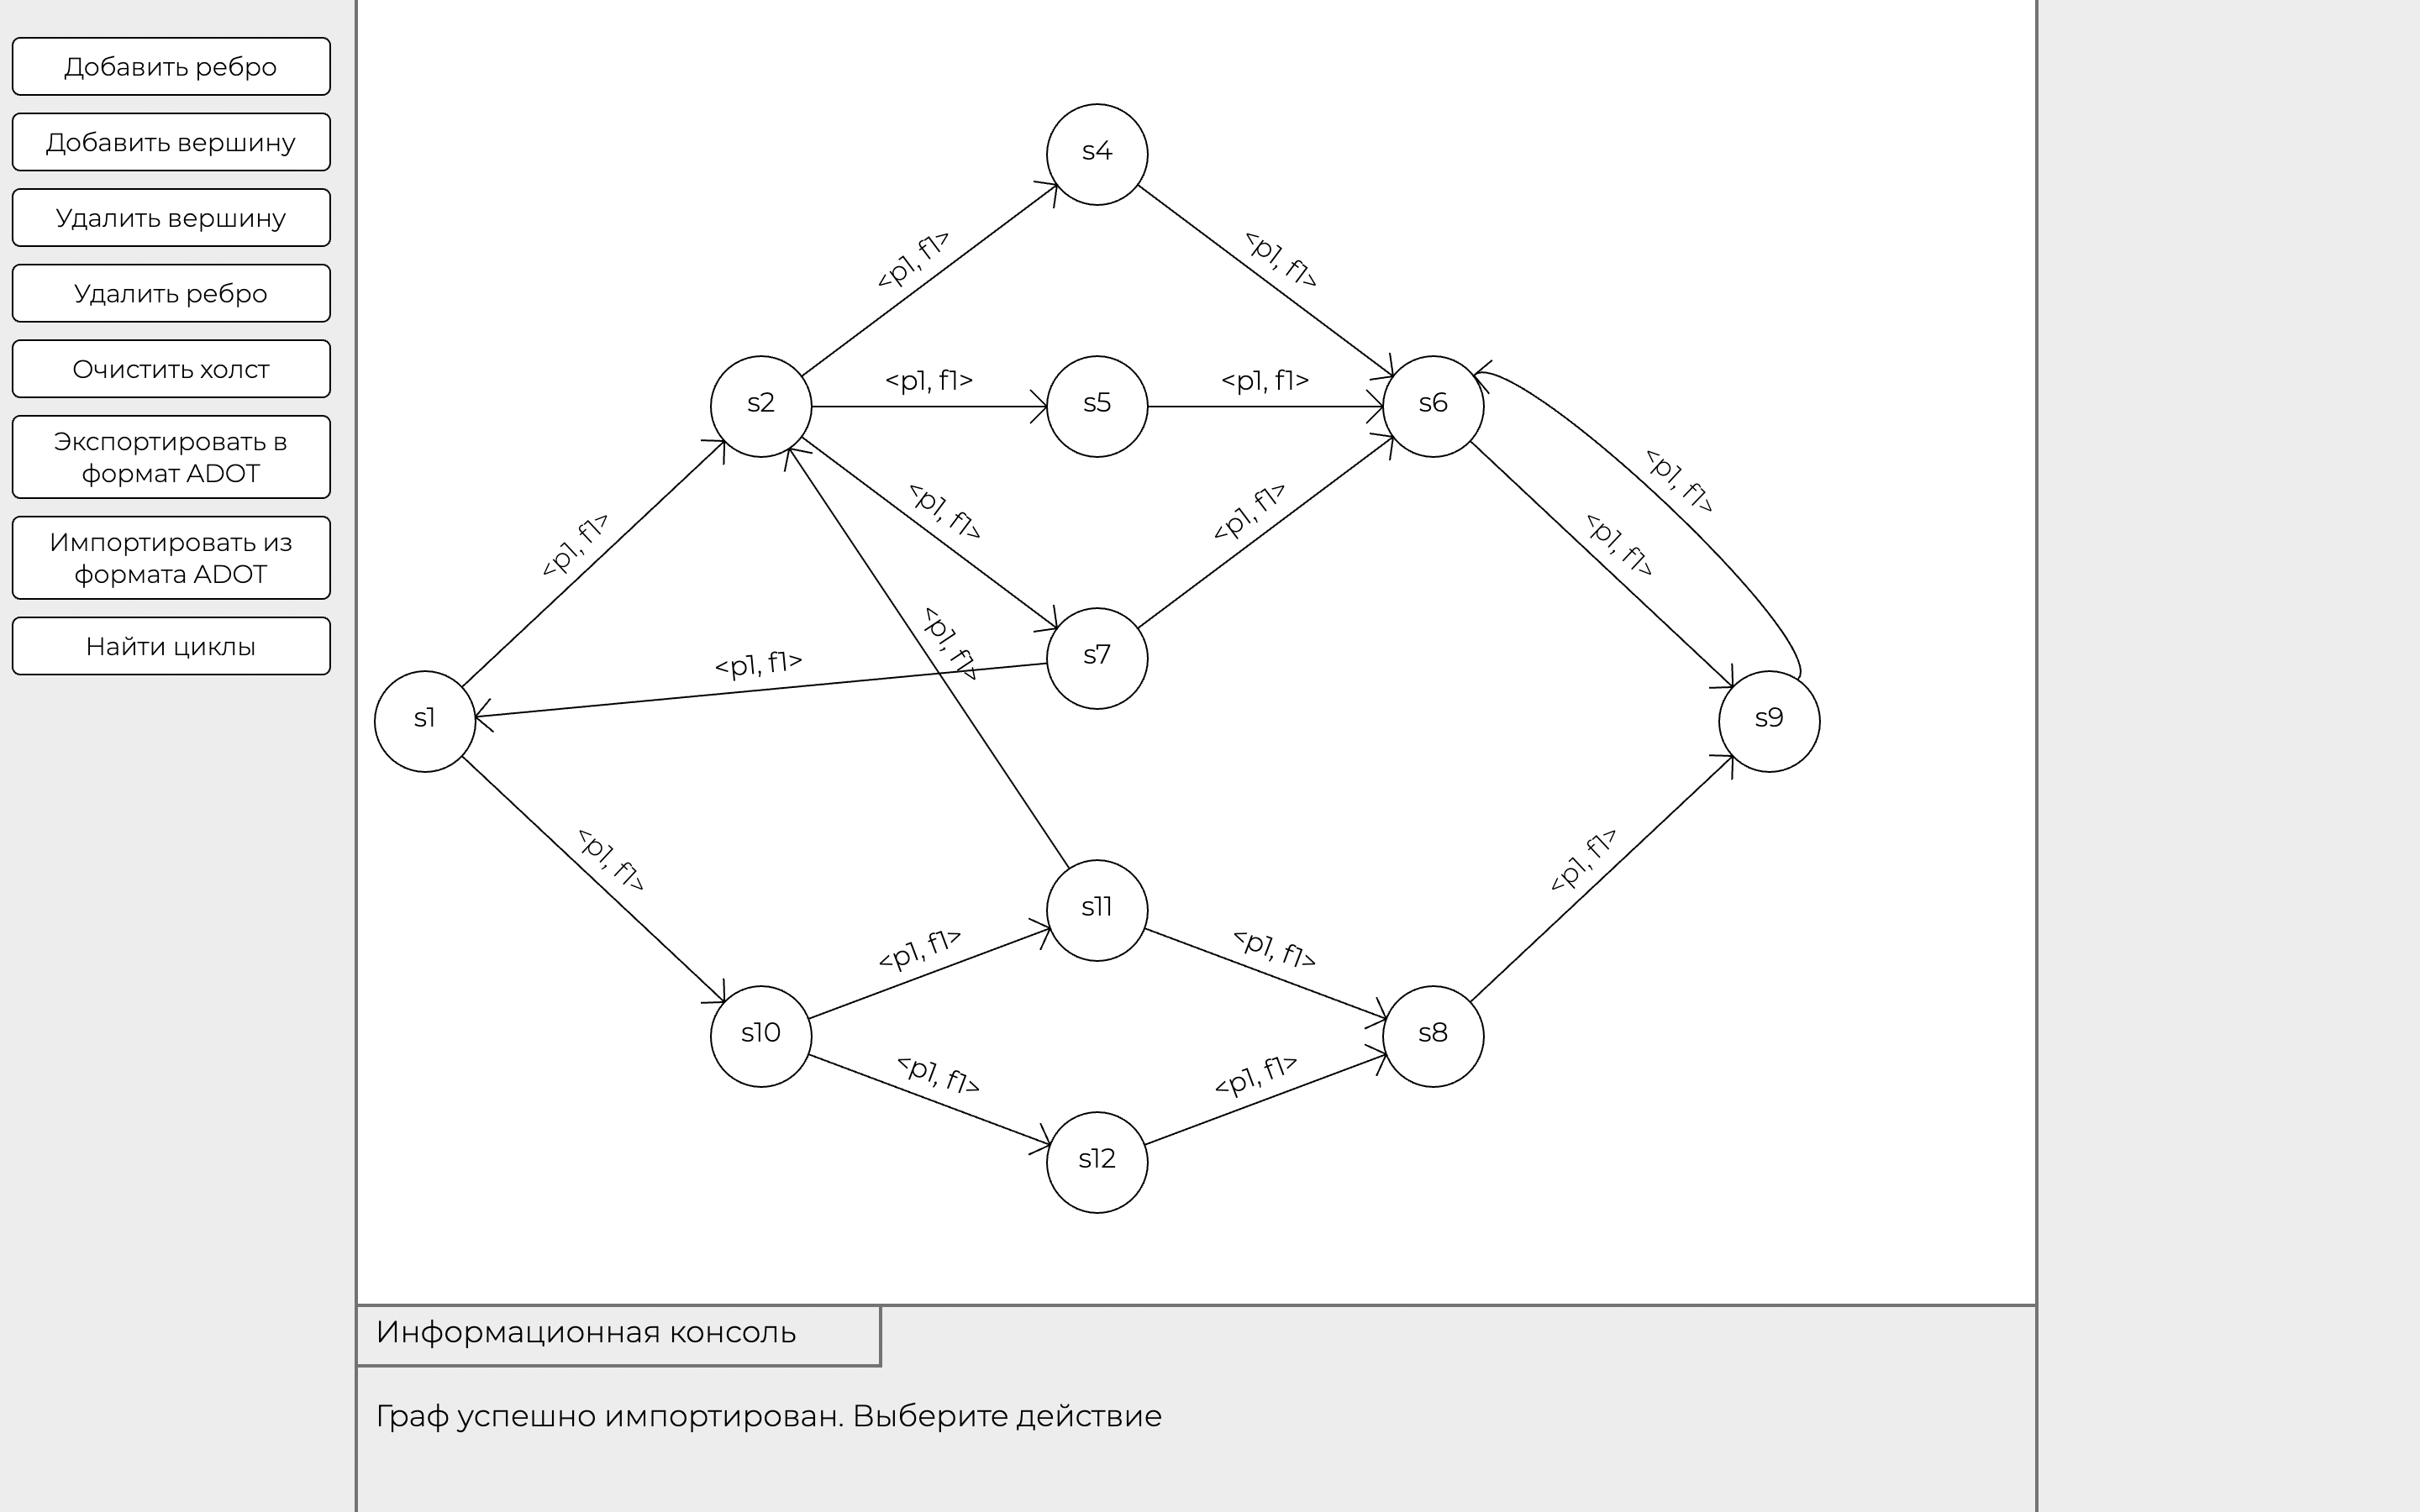
\includegraphics[width=0.9\linewidth]{images/graph_time_check.png}}
\caption{Граф для анализа скорости работы алгоритма поиска циклов}
\label{fig:example_time_check}
\end{figure} 

В результате многократного запуска поиска циклов в рассматриваемом графе были получены следующие результаты:
\begin{itemize}
\item 0.254150390625 ms
\item 0.206787109375 ms
\item 0.260986328125 ms
\item 0.236083984375 ms
\item 0.3359375 ms
\end{itemize}

Алгоритм работает достаточно быстро, однако перед выполнением поиска в глубину необходимо представить граф в виде списка смежности. Вычисление списка смежности происходит при каждом запуске поиска циклов, что не является оптимальными решением. Если графовая модель не изменяется, то повторный запуск поиска циклов будет вычислять один и тот же список смежности несколько раз. Таким образом, в качестве оптимизации алгоритма список смежности можно получать "на лету" - постепенно формировать, в случае создания графовой модели в редакторе, а в случае загрузки графовой модели получить список смежности сразу после успешной визуализации графа.